\documentclass[a4paper,11pt]{article}
\title{Getting started with iTasks}
\author{Bas Lijnse}

\usepackage{clean}
\usepackage{amssymb}
\usepackage{graphicx}

\parindent=0pt
\parskip=0.5em

\begin{document}
\maketitle
\section{Introduction}
So you have heard something about the iTask system and want to know how you can use to build a workflow support system? Then this tutorial is the right place to start. This document will walk you step-by-step through the specification of a simple example system. Because iTasks is built on top of the Clean programming language, it helps if you have some prior experience with Clean, or with related functional languages like Haskell, but it is not necessary for this tutorial. In this tutorial we are going to build a support system for managing the ever important process of keeping everybody supplied with coffee. So let's just dive right in, shall we?
\section{Setting up}
To get the iTask framework up and running we have to write just four lines of code. Start the Clean IDE and create a new file called "CoffeeTime.icl" by choosing  "File" $\rightarrow$ "New File..." from the menu. Add the following code to this file:
\begin{CleanCode}
module CoffeeTime
import iTasks

Start :: *World -> *World
Start world = startEngine [] world
\end{CleanCode}
Save this file and create a new project file called "CoffeeTime.prj" by choosing "File" $\rightarrow$ "New Project..." from the IDE's menu. Set the project's environment to "iTasks" by choosing "Environment" $\rightarrow$ "iTasks" from the menu.
\begin{figure}[h]
\centerline{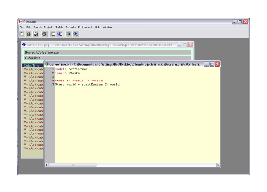
\includegraphics[width=12cm]{GettingStarted-img/ide-version1.eps}}
\caption{The Clean IDE with the CoffeeTime.icl file} \label{ide-version1}
\end{figure}
You can now build the project by selecting "Project" $\rightarrow$ "Update and Run" from the menu or pressing "Ctrl+R". After compilation, a command prompt will open showing the iTasks HTTP server in setup mode. This is shown in figure \ref{setup-server}.  The windows firewall may give a "Windows Security Alert". If this happens choose "Unblock" to allow the server listen to the HTTP port (80).
\begin{figure}[h]
\centerline{
\includegraphics[width=10cm]{GettingStarted-img/setup-server.eps}}
\caption{The server of your first iTasks application is running} \label{setup-server}
\end{figure}
If you open a browser and open the url http://localhost/ you are presented with a setup screen shown in figure \ref{setup-browser}. If you have created your project in one of the iTasks folders, like "Tutorials", "Examples" or "Assignments" all settings are set automatically and you can complete setup by clicking the "Use this default configuration" button. The server restarts and you are presented with a login screen as shown in figure \ref{login-browser}.
\begin{figure}[h]
\centerline{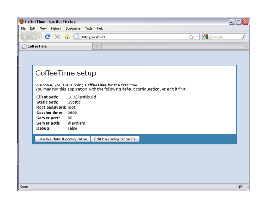
\includegraphics[width=10cm]{GettingStarted-img/setup-browser.eps}}
\caption{Setup of an iTasks application} \label{setup-browser}
\end{figure}
You can log in to your application with username "root" and password "root". This is a special superuser with full access, meant for system administration. After logging in you are presented with the default user interface of an iTask application as shown in figure \ref{empty-browser}.
\begin{figure}[h]
\centerline{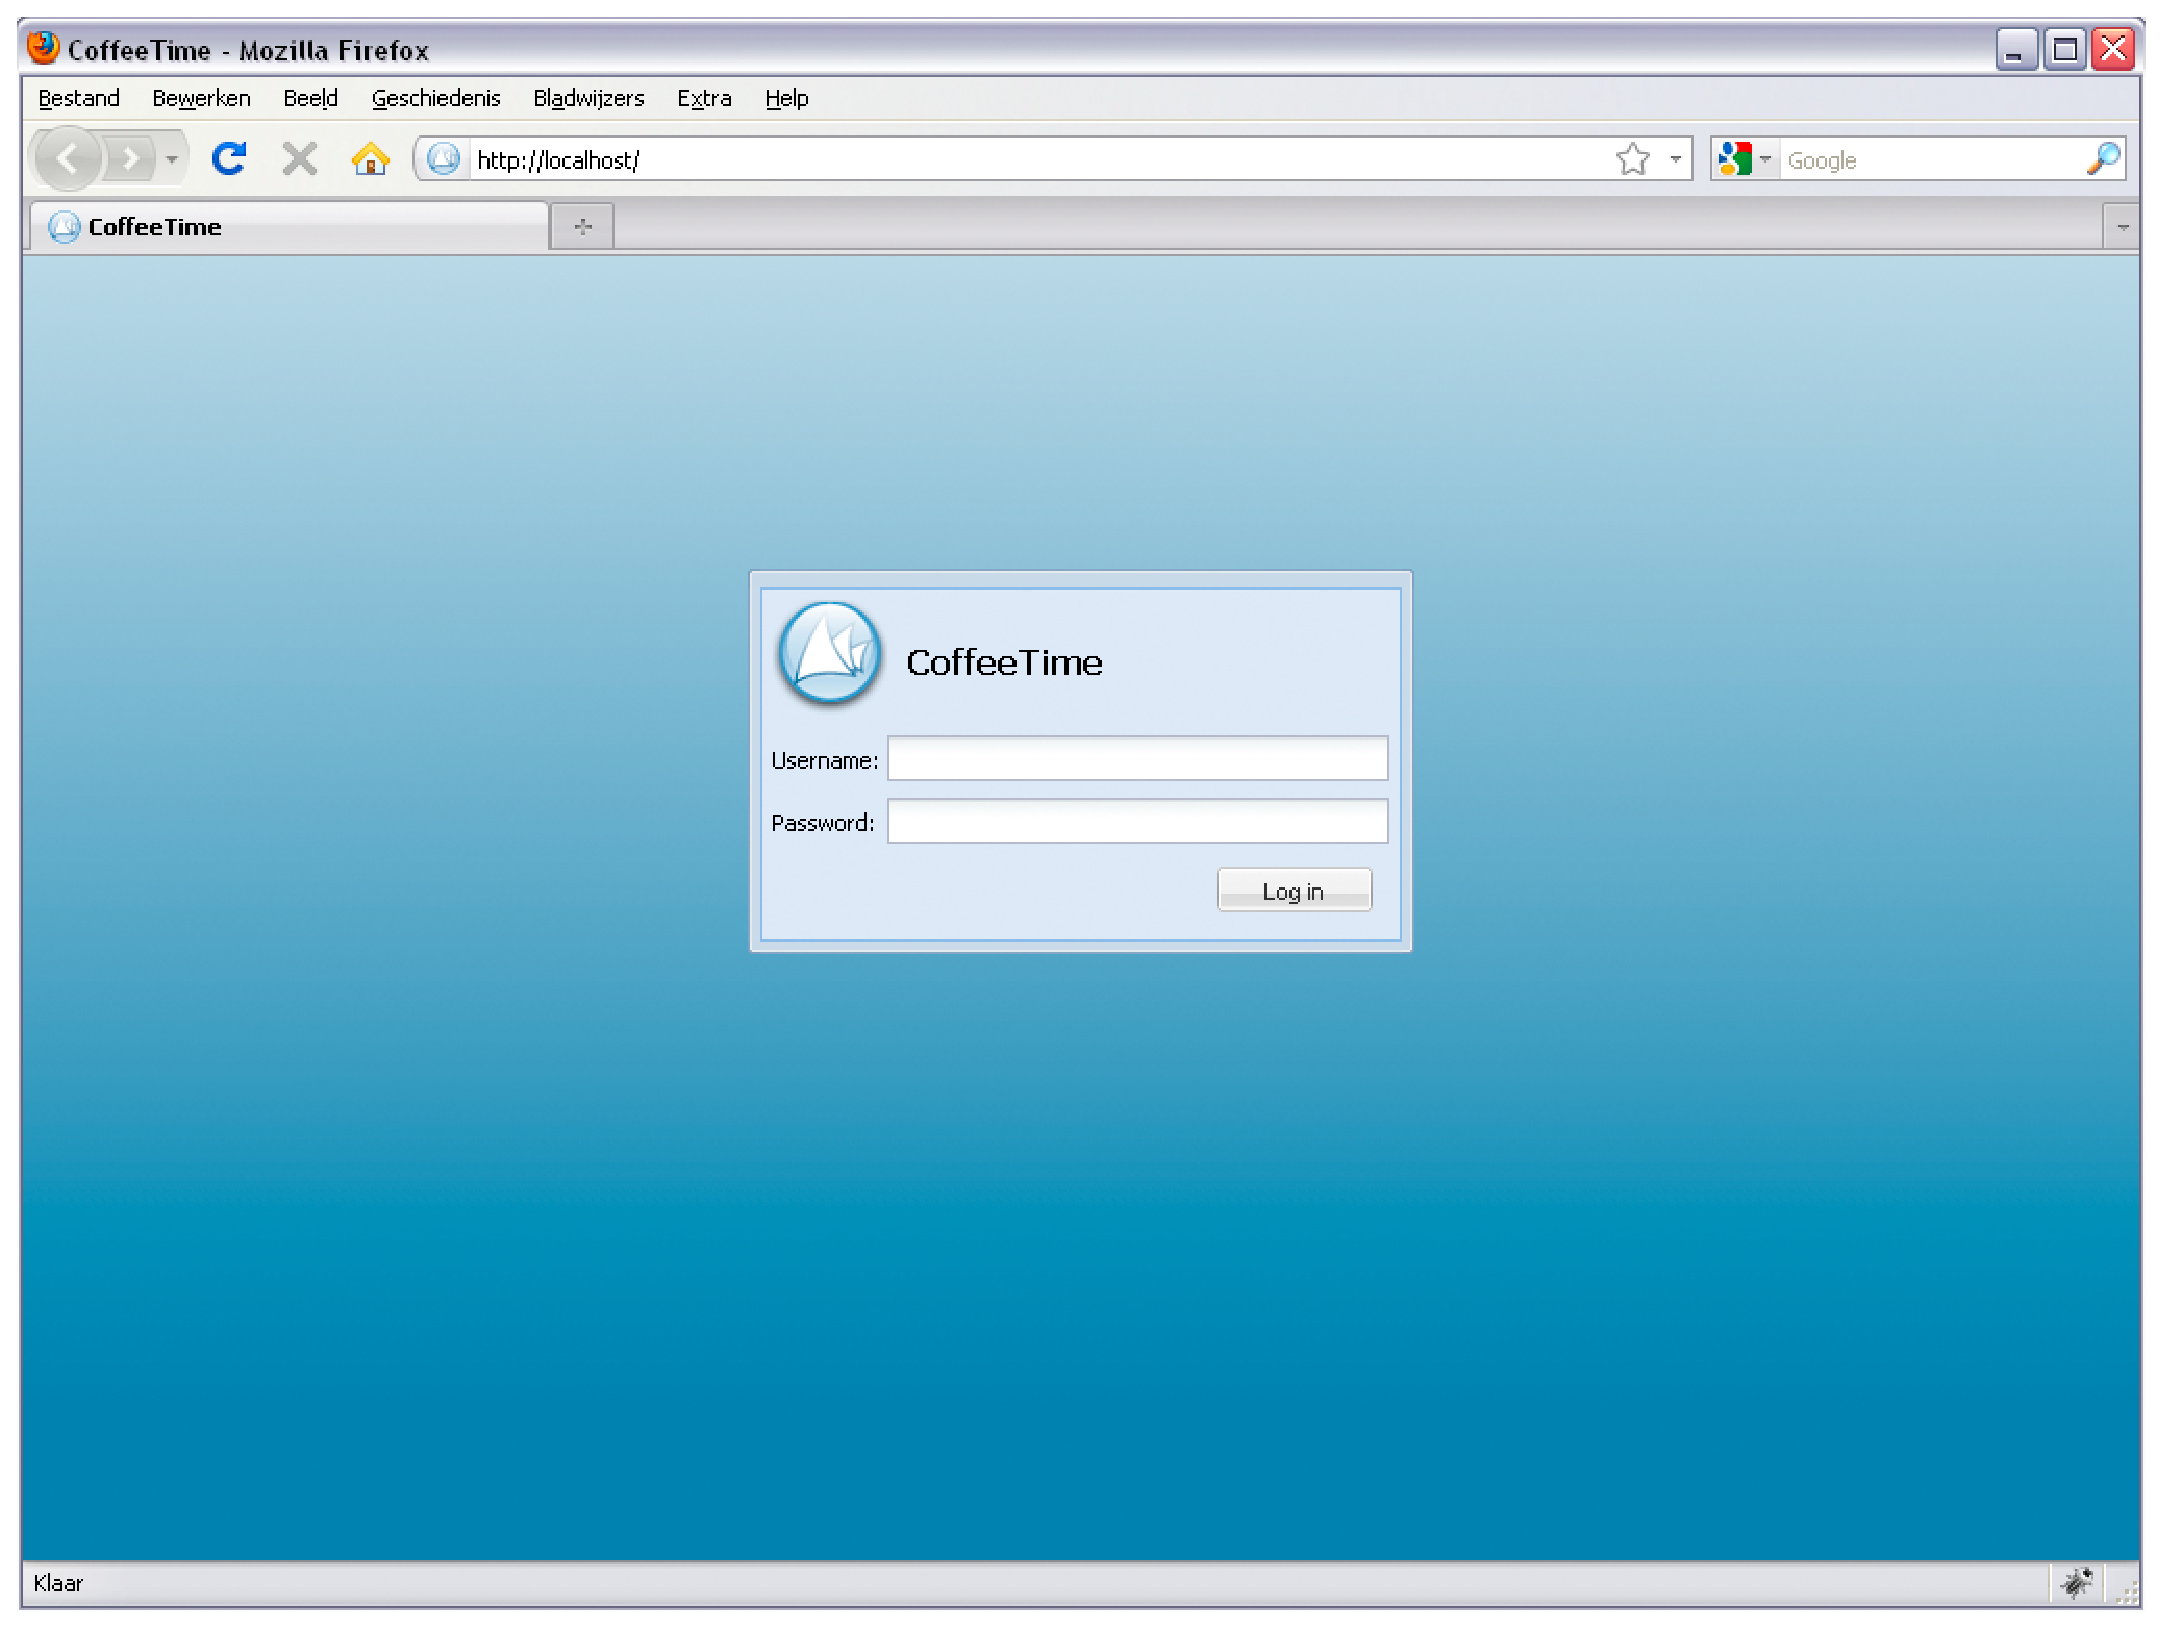
\includegraphics[width=10cm]{GettingStarted-img/login-browser.eps}}
\caption{Login screen of an iTasks application} \label{login-browser}
\end{figure}
The default user interface of an iTask application consists of three main components. The panel on the left side of the screen shows a folder hierarchy of available workflows. Users can initiate instances of these workflows based on the roles they have. The top right panel shows a user's worklist. It is a list of tasks that you are either working on or managing. The tasks in this worklist are an aggregation of all tasks assigned to you by the currently active workflow instances. The bottom right panel is the work area. In this tabbed workspace you can open tasks by double clicking them in the worklist. Further instructions and a user interface for a task are shown in the tab of an opened task.
\begin{figure}[h]
\centerline{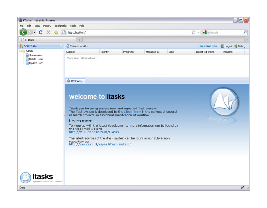
\includegraphics[width=12cm]{GettingStarted-img/empty-browser.eps}}
\caption{Default GUI of iTasks application} \label{empty-browser}
\end{figure}

When you are logged in as "root" you have access to the built-in "Admin" workflows. These are automatically added to each iTask application and can be used to manage its users. As a first exercise, open the "Admin" folder and use the "Create user" workflow for creating three users. You can choose any names you like, as long as you make three users of which you remember the username and passwords, as you will need to log in as them in a later part of this tutorial.

\section{It's Coffee time!}
So far we have seen the basic iTask framework, but except for adding users there is very little we can do with it. Let's add the most basic workflow one can think of: showing a message to the user who starts an instance of the workflow.
To do this we extend our code to:
\begin{CleanCode}
module CoffeeTime
import iTasks

Start :: *World -> *World
Start world = startEngine [workflow "Coffee time" coffeeTime] world

coffeeTime :: Task Void
coffeeTime = showMessage "Coffee time" "It's coffee time!" Void
\end{CleanCode}

We have changed two things. First we have defined a task "coffeeTime" with result type "Void". this task shows a simple string as a message. The second change is that this task is added to the engine as a toplevel worfklow. This means that users will be able to create instances of this task.To watch this code in action, you need to rebuild your application. Add the new code to the "CoffeeTime.icl" file, close the server if it is still running and press Ctrl+R to rebuild and run your project. After each rebuild your application will start with a new session and workflow database. You will therefore have to log out and log in again to be able to start your "Coffee time" workflow.

We can now start a task tells us that it's coffee time. Great! but if thats all, I'll still be thirsty tomorrow. Something has to happen when it's coffee time. A simple sketch of the  basic workflow at coffeetime would be something like the following:
\begin{enumerate}
\item Ask around to find out who else wants something to drink
\item Argue over who went to get coffee last time and decide who's turn it is this time
\item Getting the drinks if you are the unlucky one, or sit back and relax if it is someone else's turn.
\end{enumerate}
We can implement this rough sketch by updating our definition of the "coffeeTime" task definition in the CoffeeTime.icl file to the following:
\begin{CleanCode}
coffeeTime :: Task Void
coffeeTime
  =   showInstruction 
  		"Collect wishes" "Find out what everybody wants to drink" Void
  >>| showInstruction 
  		"Find victim" "Determine who gets the drinks" Void
  >>| showInstruction 
  		"Get drinks" "The unlucky one needs to go get the drinks" Void
\end{CleanCode}
This simple workfow uses the simplest sequential combinator in iTasks, the \CleanInline{>>|} combinator.  In iTasks, compound tasks are created from other tasks by using combinator functions and operators. These are functions that take other tasks as their arguments to produce a combined task. The \CleanInline{>>|} operator creates a task from two other tasks by doing its left argument first, and its right argument once the left argument is done. The result of the combination is the result of the last performed task (the rightmost one). In this case the type of the composition is \CleanInline{Void} because the type of showInstruction is \CleanInline{Void}.

\section{Who wants what?}
So far we have at least outlined the steps that are involved in getting everyone drinks at coffeetime, but the system is not very helpful yet.
It would make it a lot easier if the system coordinated the collection of everyone's drink orders. First let's define a task to collect a single order:
\begin{CleanCode}
collectOrder :: Task String
collectOrder 
	= enterChoice "Choose drink" "What do you want?" ["Coffee","Tea","Chocolate"]
\end{CleanCode}
This is our first task that produces some data. We give people a choice from a fixed set of three \CleanInline{String}s. The next thing we need to do is use this task to collect everyone's orders. But to be able to do so, we need to who who "everyone" is exactly. We can defer this problem, and assume that that information will be available at some point, so we are going to make a task that has an input argument:
\begin{CleanCode}
collectOrders :: [User] -> Task [String]
collectOrders users 
	= allTasks [(u @: (Subject "Coffee time!" @>> collectOrder) \\ u <- users]
\end{CleanCode}
In this simple task three new iTasks concepts are used. The first concept is parallel composition by the combinator \CleanInline{allTasks}. This combinator takes a list of tasks, executes them all in parallel and then produces a list of results. The type of this new task is therefore \CleanInline{[String]} (list of \CleanInline{String}) because it is a composition of a set of tasks of type \CleanInline{String}. The second is task assignment to users. The \CleanInline{@:} operator is one of the combinators that can be used to distribute work over multiple users. Its left argument is a \CleanInline{User}. Finally the \CleanInline{@>>} operator is a versatile operator which can be used to set the properties of a task. In this case we use it to change the subject.

We can now add this task in the main workflow, instead of the first intstruction task. However we will still need to get the list of users from somewhere and available for use by the \CleanInline{collectOrders} task. We do this by adding the retrieval of the user-list as an addtional step in the workflow and using the \CleanInline{>>=} combinator instead of the \CleanInline{>>|} combinator as follows:
\begin{CleanCode}
coffeeTime :: Task Void
coffeeTime
  =   getUsers
  >>= \users -> collectOrders users
  >>| showInstruction "Find victim" "Determine who gets the drinks"
  >>| showInstruction "Get drinks" "The unlucky one needs to go get the drinks"
\end{CleanCode}
The \CleanInline{>>=} combines two tasks sequentially and passes the result of the first task as argument to the second. The \CleanInline{\\users ->} part\footnote{Instead of a lambda you can type a backslash in Clean source files} that comes after the \CleanInline{>>=} combinator turns what comes after it into a parameterized task. What we gain from this is that we can give the result of the previous task a name and use that name to pass the result to later tasks. In this case to \CleanInline{collectOrders}. If you run the current version of this worfklow you can see how a multi user workflow in iTasks works. You will have to log in as all the users you created in the beginning of the tutorial.

Currently our workflow is a little bit too demanding. We have to say what we want to drink. But what if we are not thirsty? We can make the workflow definition a little more friendly by making the result type of the \CleanInline{collectOrder} task optional. The result type of the \CleanInline{collectOrders} task then needs to be changed to a list of optional results. We will change the code to let the choice of drinks be preceded by the question whether someone wants something to drink. We change the specification to the following:
\begin{CleanCode}
collectOrders :: [User] -> Task [Maybe String]
collectOrders users 
	= allTasks [u @: (Subject "Coffee time!" @>> collectOrder) \\ u <- users]

collectOrder :: Task (Maybe String)
collectOrder
	= requestConfirmation "Coffee time!" "It is coffee time, do you want something?"
	>>= \yes -> if yes
		(enterChoice "Choose drink" "What do you want" ["Coffee","Tea","Chocolate"]
		>>= \choice -> return (Just choice))
		(return Nothing)
\end{CleanCode}
Again, several new things are happening. We use the boolean result of the \CleanInline{requestConfirmation} task to decide what task comes after it.
The \CleanInline{if} function has three arguments. The first is the boolean value that determines which of the next two arguments is chosen. When the answer to the first question is yes, the second task is the orginal choice followed by a task that returns the result wrapped as \CleanInline{Just} the result. If the answer is no, the result \CleanInline{Nothing} is returned.
\section{Making an order list, and getting drinks}
Now that we know that results from one tasks can be used in subsequent tasks, we can use the information we got from collecting everybody's orders to use in the last two tasks of the main workflow. However, the information we have is not easily grouped. The first task of the main workflow gave us a list of all usernames, and the second task gives us a list of optional drink orders. What we need, is a combined list of names and orders for everybody who wants something. To do this we add the following code to our specification:
\begin{CleanCode}
orderlist :: [User] [Maybe String] -> [(User,String)]
orderlist users orders
 = [(user, fromJust order) \\ user <- users & order <- orders | isJust order]
\end{CleanCode}
Contrary to the code we have so far, this is not a task specification. Because the iTasks combinator language is embedded in the Clean programming language, we can mix our tasks with ordinary function definitions. In our main workflow, we change the last two tasks to tasks that take the order list we construct with the new function as their argument.
\begin{CleanCode}
coffeeTime :: Task Void
coffeeTime
	=   getUserNames
	>>= \users ->  collectOrders users
	>>= \orders -> determineWhoGoes (orderlist users orders)
	>>= \victim -> goGetCoffee victim (orderlist users orders)
\end{CleanCode}

To finish the main workflow we have also already added another argument to the final task. This is the user who is selected to get the drinks.
To complete the full task definition we add the last bit of code. The definition of \CleanInline{determineWhoGoes} and \CleanInline{goGetCoffee} as follows:
\begin{CleanCode}
determineWhoGoes :: [(User,String)] -> Task User
determineWhoGoes orders = randomChoice [user \\ (user,_) <- orders]

goGetCoffee :: User [(User,String)] -> Task Void
goGetCoffee user orders
	= user @:
	(Subject "Get coffee" @>> 
		(showInstructionAbout 
			"Coffee orders"
			"You have been chosen to get the following drinks"
			orders
			>>| stop
		)                        
	)
\end{CleanCode}
In these tasks a random username is chosen from the list of all usernames in the drink orders, and is the order list presented to that unlucky user.
\section{Conclusions}
In this tutorial we have step-by-step created a simple support system for a "coffee time" workflow. Although we have only discussed the presented code superficially, it should give you a basic idea of what  building workflow support systems with iTasks is like.
\appendix
\newpage
\section{The complete source code}
This is it. A complete workflow support system for co\"ordinating a core process of many organizations in just over forty lines of code.
\begin{CleanCode}
module CoffeeTime
import iTasks

Start :: *World -> *World
Start world = startEngine [workflow "Coffee time" coffeeTime] world

coffeeTime :: Task Void
coffeeTime
	=   getUserNames
	>>= \users ->  collectOrders users
	>>= \orders -> determineWhoGoes (orderlist users orders)
	>>= \victim -> goGetCoffee victim (orderlist users orders)

orderlist :: [User] [Maybe String] -> [(User,String)]
orderlist users orders
	= [(user, fromJust order) \\ user <- users & order <- orders | isJust order]

collectOrders :: [User] -> Task [Maybe String]
collectOrders users 
	= allTasks [u @: (Subject "Coffee time!" @>> collectOrder) \\ u <- users]

collectOrder :: Task (Maybe String)
collectOrder
	= requestConfirmation "Coffee time!" "It is coffee time, do you want something?"
	>>= \yes -> if yes
		(enterChoice "Choose drink" "What do you want" ["Coffee","Tea","Chocolate"]
		>>= \choice -> return (Just choice))
		(return Nothing)

determineWhoGoes :: [(User,String)] -> Task User
determineWhoGoes orders = randomChoice [user \\ (user,_) <- orders]

goGetCoffee :: User [(User,String)] -> Task Void
goGetCoffee user orders
	= user @:
	(Subject "Get coffee" @>> 
		(showInstructionAbout 
			"Coffee orders"
			"You have been chosen to get the following drinks"
			orders
			>>| stop
		)                        
	)

\end{CleanCode}
\end{document}
